\documentclass[11pt,a4paper]{article}
\usepackage[margin=22mm]{geometry}
\usepackage[T1]{fontenc}
\usepackage{lmodern,microtype,amsmath,amssymb,booktabs,graphicx,float,array,xcolor}
\usepackage{xurl}
\usepackage[hidelinks]{hyperref}
\usepackage{fancyhdr}
\pagestyle{fancy}\fancyhf{}\fancyhead[L]{Roy-inspired DCT rainfall reconstruction}\fancyhead[R]{Technical note}\fancyfoot[C]{\thepage}\fancyfoot[R]{\hyperlink{contents}{Contents}}
\fancypagestyle{plain}{\fancyhf{}\fancyfoot[C]{\thepage}\fancyfoot[R]{\hyperlink{contents}{Contents}}\renewcommand{\headrulewidth}{0pt}}
\setlength{\headheight}{14pt}
\setlength{\parindent}{0pt}\setlength{\parskip}{6pt}
\newcommand{\norm}[1]{\left\lVert#1\right\rVert}
\newcommand{\R}{\mathbb R}
\newcommand{\J}{\mathcal J}
\title{Rainfall reconstruction with a sparse DCT prior\\\large Formulation, numerical solver, and the 100-patch experiment}
\author{Implementation and saved-run audit}
\date{24 September 2026}
\begin{document}
\maketitle
\begin{abstract}
This note documents the implemented nonlinear adaptation of the no-dynamics formulation of Roy, Gishkori and Leus (2016). It connects the rainfall objective to the outer linearization and inner ADMM updates, states the exact stopping rules, and audits the saved 100-patch experiment. All inner subproblems met their numerical stopping tests, but every patch exhausted 50 outer iterations. The accuracy and runtime results therefore describe iteration-limited outputs, not converged nonlinear minimizers. No reconstructions were rerun to prepare this note.
\end{abstract}
\clearpage\hypertarget{contents}{}\tableofcontents\clearpage
\section{Objective and connection to Roy et al.}
Roy et al., Section 5.3.3, Eqs.~(26)--(27), use a linear, no-dynamics model and an orthonormal basis $\Psi$ \cite{roy}:
\begin{equation}
 \min_{\Psi c\ge0}\norm{y-\Phi\Psi c}_{R^{-1}}^2+\lambda\norm{c}_1,
 \qquad u=\Psi c.\label{eq:roy}
\end{equation}
Since $D=\Psi^T$ is orthonormal, $c=Du$. With $R=\sigma^2 I$, the identical linear objective in rainfall coordinates is
\begin{equation}
 \min_{u\ge0}\frac{1}{\sigma^2}\norm{y-\Phi u}_2^2+\lambda\norm{Du}_1.
\end{equation}
Our experiment retains the penalty and constraint, but replaces $\Phi u$ by the existing nonlinear ITU attenuation model:
\begin{equation}
 \boxed{\min_{u\ge0}\J(u),\qquad
 \J(u)=\frac{1}{\sigma^2}\norm{y-F(u)}_2^2+\lambda\norm{Du}_1.}\label{eq:objective}
\end{equation}
\textbf{This is the same structural formulation, but a different measurement experiment.} It becomes the same linear optimization problem when the forward map is linear and the basis and data conventions agree. The present ITU version is generally nonconvex. Roy et al. explicitly suggest iterative linearization as a nonlinear extension; the specific ADMM/CG, damping and stopping implementation documented here is ours.

Each patch is reconstructed independently. There is no temporal prediction, Kalman covariance update, previous-map penalty, learned basis, or estimated spatial covariance in this implementation.
\clearpage
\section{Variables, measurements and spatial representation}
\begin{tabular}{p{.16\linewidth}p{.77\linewidth}}\toprule
Symbol & Meaning\\\midrule
$u\in\R^N$ & Rainfall at $N=HW$ pixels, in the repository's mm/h convention; $H$ rows and $W$ columns.\\
$y\in\R^M$ & Observed/simulated link attenuations in dB.\\
$L_{\ell i}$ & Length in km of link $\ell$ inside pixel $i$; zero for untraversed pixels.\\
$k_\ell,\alpha_\ell$ & Fixed ITU power-law coefficients for link $\ell$.\\
$D$ & Orthonormal, separable 2D DCT-II analysis operator; $D^TD=I$.\\
$\lambda$ & Weight of the sum of absolute DCT coefficients, including the constant mode.\\
$\sigma^2$ & Shared residual variance/weight; $R=\sigma^2 I$.\\\bottomrule
\end{tabular}
\begin{equation}
 F_\ell(u)=\sum_{i=1}^N L_{\ell i}k_\ell u_i^{\alpha_\ell}.
\end{equation}
The residual term uses link attenuation directly. It is not divided by link length, link count, or pixel count. Length-normalized residuals used in comparison tables are separate evaluation metrics.

For column $j=0,\ldots,W-1$ and row $i=0,\ldots,H-1$, a basis pattern is
\begin{equation}
 \psi_{pq}(j,i)=a_p^{(W)}a_q^{(H)}
 \cos\!\frac{\pi p(j+1/2)}{W}\cos\!\frac{\pi q(i+1/2)}{H},
\end{equation}
where $p=0,\ldots,W-1$, $q=0,\ldots,H-1$, $a_0^{(n)}=1/\sqrt n$, and $a_r^{(n)}=\sqrt{2/n}$ for $r>0$. There are $N$ patterns, each with $N$ pixel values. Flattening a pattern gives a column of $\Psi=D^T$. The implementation applies transforms instead of storing these columns.

All frequencies are available; coefficients may be positive or negative. A small $\ell_1$ norm encourages a sparse coefficient representation but is not an explicit smoothness penalty and does not preferentially penalize high frequencies. Nonnegativity applies to the reconstructed field. Choosing 2D DCT-II is an explicit implementation convention; the paper does not unambiguously resolve 2D versus flattened 1D DCT in its example.
\section{Parameter choices and initialization}
Section 5.3.3 of Roy et al. uses $\lambda=2$, DCT, linear coefficients $a=b=1$, and noise variance $\sigma_e^2=10^{-5}$ \cite{roy}. We transferred $\lambda=2$ and $\sigma^2=10^{-5}$ without tuning. Thus $\sigma=\sqrt{10^{-5}}\simeq0.0031623$, not $10^{-5}$. In our model this is in attenuation units; it is a weighting choice, not an estimate of noise in the present dataset. Different units, grids and nonlinear coefficients mean the transfer is not statistically calibrated.

All 100 runs start with $u_{0,i}=0.6$ mm/h for every pixel $i=1,\ldots,N$. The initialization is exactly 0.6, not 0.61; the previous vector notation used a bold one to mean a vector of ones. Only the constant DCT coefficient is initially nonzero. This positive constant is our choice, not a value established by Roy's linear experiment. Initialization can change nonlinear trajectories and local solutions; sensitivity to other starts has not been tested.
\clearpage
\section{Which software and which class of problem?}
\textbf{There is no optimization modeling language in the implementation used for these runs.} Python code expresses the operators and updates directly. NumPy supplies array operations. SciPy supplies \texttt{fft.dctn}/\texttt{idctn} with \texttt{type=2, norm="ortho"}, sparse CSR matrices, \texttt{LinearOperator}, and \texttt{sparse.linalg.cg} \cite{dct,cg}. Custom code implements ADMM and the nonlinear outer loop.

CVXPY plus OSQP was an earlier proposed alternative, not the executed solver. CVXPY is a Python modeling layer and OSQP solves convex quadratic programs. The paper reports CVX (MATLAB modeling layer) with SeDuMi for its convex estimation problems. Neither CVXPY, OSQP nor SeDuMi is called by our Roy implementation.

ADMM is suited to convex objectives split into readily solvable pieces with linear equality constraints. Here, the pieces are quadratic fitting, the nonsmooth $\ell_1$ penalty, and nonnegativity. CG solves the positive-definite linear system in one of the ADMM updates; it does not directly solve the complete constrained problem.
\subsection{Why custom ADMM rather than OSQP?}
The reason was the representation of the large DCT operator. OSQP's standard Python interface takes explicit sparse matrices $P$ and $A$, not a user-supplied DCT multiplication function \cite{osqp}. A straightforward QP with $-t\le Dx\le t$ would put the dense DCT matrix into those constraints. At 250,000 pixels, that matrix alone contains 62.5 billion entries (500 GB as dense float64).

Our split applies $D$ and $D^T$ using fast transforms, and uses $D^TD=I$ to simplify the quadratic update. SciPy supplies these transforms and CG; NumPy supplies the array arithmetic. The ADMM updates, residual checks, adaptive penalty and nonlinear outer loop are custom code. These libraries are sufficient building blocks, but do not automatically verify the complete algorithm.

OSQP remains a valid option for a small explicit version of each convex subproblem, and a useful independent validation reference. A specially structured reformulation might also avoid the naive dense basis. We did not benchmark those alternatives, so this choice is not evidence that our solver is faster or more accurate. Custom code entails more implementation and validation responsibility. OSQP alone would still not solve the full nonlinear objective: an outer nonlinear strategy would remain necessary.
\clearpage
\subsection{Why the subproblem is convex}
Multiply Eq.~\eqref{eq:objective} by the positive constant $\sigma^2/2$:
\begin{equation}
 f(u)=\tfrac12\norm{y-F(u)}_2^2+\beta\norm{Du}_1,
 \qquad \beta=\lambda\sigma^2/2=10^{-5}.\label{eq:scaled}
\end{equation}
This preserves minimizers and the relative weighting. Reported objective values use $\J=2f/\sigma^2$.

At outer iteration $k$, hold $J_k$ and $b_k$ fixed and solve
\begin{equation}
 \min_{x\ge0} Q_k(x)=\tfrac12\norm{J_kx-b_k}_2^2
 +\beta\norm{Dx}_1+\tfrac\mu2\norm{x-u_k}_2^2.\label{eq:sub}
\end{equation}
The quadratic part has Hessian $J_k^TJ_k+\mu I$. For any $w$,
\[
 w^T(J_k^TJ_k+\mu I)w=\norm{J_kw}_2^2+\mu\norm{w}_2^2\ge0.
\]
The $\ell_1$ norm composed with a linear map is convex; $x\ge0$ defines a convex set. Consequently the subproblem is convex, and is strongly convex for our $\mu=10^{-3}>0$.

Strictly, the absolute-value objective is nonsmooth, not a quadratic polynomial. An equivalent convex QP introduces $t$ and replaces $\norm{Dx}_1$ by $\mathbf1^Tt$, with $-t\le Dx\le t$. Its objective is quadratic and its constraints linear. ADMM exploits this structure without assembling a generic QP.

The full nonlinear squared residual need not be convex. Linearizing $F$ makes each subproblem convex; it does not make the original objective convex or guarantee its global minimum. Damping is a local step-selection device, not an extra term in the reported original objective.
\clearpage
\section{One outer iteration: approximate, propose, check}
\subsection{Linearize the attenuation model}
For a change $d$, use
\[
 F(u_k+d)\approx F(u_k)+J_kd,\qquad
 (J_k)_{\ell i}=L_{\ell i}k_\ell\alpha_\ell(u_{k,i})^{\alpha_\ell-1}.
\]
The implementation evaluates the power in the derivative at $\max(u_{k,i},10^{-6})$. This avoids divergent derivatives at zero when $\alpha_\ell<1$, and zero sensitivity at dry pixels when $\alpha_\ell>1$. The actual forward model is not floored. Near the boundary this is a safeguarded derivative rather than the exact derivative, limiting stationarity claims.
\subsection{Find the candidate map}
The damped step subproblem is
\[
 \min_{d:\,u_k+d\ge0}
 \tfrac12\norm{y-F(u_k)-J_kd}_2^2
 +\beta\norm{D(u_k+d)}_1+\tfrac\mu2\norm d_2^2.
\]
Set $x=u_k+d$ and $b_k=y-F(u_k)+J_ku_k$. This gives Eq.~\eqref{eq:sub}. Only the forward model is linearized; the sparsity penalty and constraint remain intact. ADMM approximately solves it, returning a feasible candidate $v_k$. Set $d_k=v_k-u_k$.
\subsection{Backtrack on the original nonlinear objective}
Define the predicted improvement using the damped subproblem,
\[
 P_k=f(u_k)-Q_k(v_k).
\]
Try $s=1,1/2,1/4,\ldots$ and accept the \emph{first} trial satisfying
\begin{equation}
 f(u_k+s d_k)\le f(u_k)-10^{-4}s\max(0,P_k).\label{eq:armijo}
\end{equation}
There are at most 30 trial evaluations (through $s=2^{-29}$). If $P_k\le0$, the code's condition requires nonincrease rather than strict decrease. Both endpoints are nonnegative, so every trial is feasible. Set $u_{k+1}=u_k+s d_k$ and relinearize for the next outer iteration.

Damping discourages a large proposed change; backtracking checks the proposal against the actual nonlinear objective. It is not an exact minimization over step sizes. In the saved experiment all 5,000 updates accepted $s=1$; the smaller trial steps were never needed.

The exact linear mode uses $\mu=0$ and a single ADMM subproblem. That mode was not used for these 100 patches.
\clearpage
\section{Inner ADMM: how the candidate is found}
Introduce $z=Dx$ and $v=x$, with $v\ge0$. Equation~\eqref{eq:sub} is equivalent to
\[
 \min_{\substack{x,z,v\\v\ge0}}\tfrac12\norm{J_kx-b_k}^2+
 \tfrac\mu2\norm{x-u_k}^2+\beta\norm z_1,
 \quad z=Dx,\quad v=x,
\]
where only $v$ is constrained nonnegative; $x$ and $z$ are unrestricted. ADMM uses scaled dual variables $a,c$ to accumulate disagreement. Its augmented expression, up to terms constant in the primal updates, is
\begin{align*}
 &\tfrac12\norm{J_kx-b_k}^2+\tfrac\mu2\norm{x-u_k}^2+\beta\norm z_1\notag\\
 &\hspace{8mm}+\tfrac\rho2\norm{Dx-z+a}^2+\tfrac\rho2\norm{x-v+c}^2,
 \qquad v\ge0.
\end{align*}
At each outer call initialize $x=v=u_k$, $z=Du_k$, $a=c=0$, and $\rho=1$. Dual variables and $\rho$ are reset between outer calls. Within ADMM, repeat:
\begin{enumerate}
\item \textbf{Quadratic $x$ update.} Hold all other variables fixed and solve
\begin{align}
 [J_k^TJ_k+(\mu+2\rho)I]x
 &=J_k^Tb_k+\mu u_k\notag\\
 &\quad+\rho[D^T(z-a)+v-c].\label{eq:cg}
\end{align}
The $\ell_1$ term is constant in this update because it depends on $z$. Nonnegativity is enforced through the separate $v$ update.
\item \textbf{Sparse coefficient update.} With $w=Dx+a$, use
\[
 z_i=\operatorname{sign}(w_i)\max(|w_i|-\beta/\rho,0).
\]
This soft threshold shrinks large coefficients and zeros small ones; it is the exact minimizer of $\beta\norm z_1+\frac\rho2\norm{Dx-z+a}^2$.
\item \textbf{Nonnegative update.} Set $v=\max(x+c,0)$ elementwise. This projection happens inside optimization, not as final cosmetic clipping.
\item \textbf{Dual updates.} Set $a\leftarrow a+Dx-z$ and $c\leftarrow c+x-v$. These variables retain pressure to resolve disagreement.
\end{enumerate}
The $x$ system is symmetric positive definite because $\mu+2\rho>0$. SciPy CG is warm-started from the previous inner $x$ and uses a diagonal inverse preconditioner with entries $[\sum_\ell J_{\ell i}^2+\mu+2\rho]^{-1}$. The matrix action is $J_k^T(J_kw)+(\mu+2\rho)w$; neither $J_k^TJ_k$ nor $D$ is stored densely. Every 25 ADMM iterations, residual balancing doubles $\rho$ if primal residual exceeds ten times dual, or halves it for the reverse, within $[10^{-10},10^8]$; scaled duals are adjusted accordingly.
\clearpage
\section{Stopping rules and numerical settings}
\subsection{CG stopping within each ADMM iteration}
For $Hx=q$ in Eq.~\eqref{eq:cg}, SciPy tests
\[
 \norm{q-Hx}_2\le 10^{-8}\norm q_2.
\]
Absolute tolerance is zero and the maximum is 500 CG iterations per call. A nonzero CG return code, or a nonfinite iterate, makes the inner solve fail. CG residual magnitudes are not saved, so their final tolerance margins cannot be reconstructed from the logs.
\subsection{ADMM stopping within each outer iteration}
After each update let $(z^-,v^-)$ be the previous inner values. The saved residuals are
\begin{align*}
 r_{\rm p}&=\sqrt{\norm{Dx-z}_2^2+\norm{x-v}_2^2},\\
 r_{\rm d}&=\rho\norm{D^T(z-z^-)+(v-v^-)}_2.
\end{align*}
With $\epsilon_a=10^{-6}$, $\epsilon_r=10^{-5}$ and $N$ pixels, the code uses
\begin{align*}
 \epsilon_{\rm p}&=\sqrt{2N}\epsilon_a+
 \epsilon_r\max\{\sqrt2\norm x_2,\sqrt{\norm z_2^2+\norm v_2^2}\},\\
 \epsilon_{\rm d}&=\sqrt N\epsilon_a+
 \epsilon_r\rho\norm{D^Ta+c}_2.
\end{align*}
Both $r_{\rm p}\le\epsilon_{\rm p}$ and $r_{\rm d}\le\epsilon_{\rm d}$ are required. The primal test checks agreement; the dual test checks the associated stationarity residual. These are optimization tolerances, not rainfall errors. At most 2,000 ADMM iterations are allowed per outer call. The feasible $v$ is returned. An inner failure stops the outer solver as unsuccessful (an accepted candidate can already have been stored before this failure check).
\subsection{Outer stopping}
For a successfully solved subproblem, define
\begin{equation}
 \eta_k=\frac{\norm{v_k-u_k}_2}{\max(1,\norm{u_k}_2)}.
\end{equation}
The nonlinear convergence flag requires $\eta_k\le10^{-5}$. It uses the \emph{full proposed step}, not the shortened accepted step; a tiny backtracking step alone cannot trigger success. This is a local fixed-point test, not a global-optimality or rainfall-accuracy certificate. The derivative safeguard further limits exact nonlinear stationarity claims.

The cap is 50 outer iterations. Additional failure exits cover a nonfinite Jacobian, CG/ADMM failure and exhausted backtracking. A converged inner solve with a tiny full step is accepted as a fixed point even if the line search does not accept a trial. There is no outer relative-objective-decrease stopping test in this implementation.

The fixed parameters are $\lambda=2$, $\sigma^2=10^{-5}$, $\mu=10^{-3}$, initial $\rho=1$, derivative floor $10^{-6}$, line-search constant $10^{-4}$, and initial rainfall $0.6$ mm/h. Only $\lambda$ and $\sigma^2$ were transferred from the paper's linear experiment; the remaining numerical settings are implementation choices.
\clearpage
\section{What happened in the 100 saved runs?}
All 100 runs report \texttt{success=false}, \texttt{stop\_reason=max\_outer}, and 50 outer iterations. All 5,000 inner solves report \texttt{admm\_residuals}; none stopped on a CG failure or inner iteration cap. Every outer step was accepted at full size.
\begin{table}[H]\centering\small\begin{tabular}{lrrrr}\toprule Quantity & Minimum & Median & Mean & Maximum\\\midrule
Final relative full step & 0.0016689 & 0.0032803 & 0.0031542 & 0.0034254 \\
Step / outer tolerance & 166.89 & 328.03 & 315.42 & 342.54 \\
Final primal / tolerance & 0.0016914 & 0.011601 & 0.011581 & 0.020437 \\
Final dual / tolerance & 0.98462 & 0.99183 & 0.99162 & 0.99977 \\
ADMM iterations per patch & 11171 & 12632 & 12604 & 13854 \\
CG iterations per patch & 30878 & 38750 & 61845 & 2.0835e+05 \\
\bottomrule\end{tabular}
\caption{Final-outer-step residual ratios and total work per patch. A residual/tolerance ratio must be at most one to pass.}\end{table}
The median final step was $0.0032803$, or about $0.328\%$ of the field norm, versus a requested $0.001\%$. Final outer steps were 166.9--342.5 times the threshold. These ratios do \emph{not} measure distance to the optimum and do not predict how many further iterations are needed.

The last inner solves passed comfortably on primal agreement (ratios at most 0.02044) and just passed on the dual criterion (0.98462--0.99977). Across all 5,000 inner solves, the maximum primal ratio was 0.08265 and maximum dual ratio 0.999994. There were 1,260,373 ADMM iterations and 6,184,482 CG iterations in total, or about 252 ADMM iterations per outer call on average.
\begin{figure}[H]\centering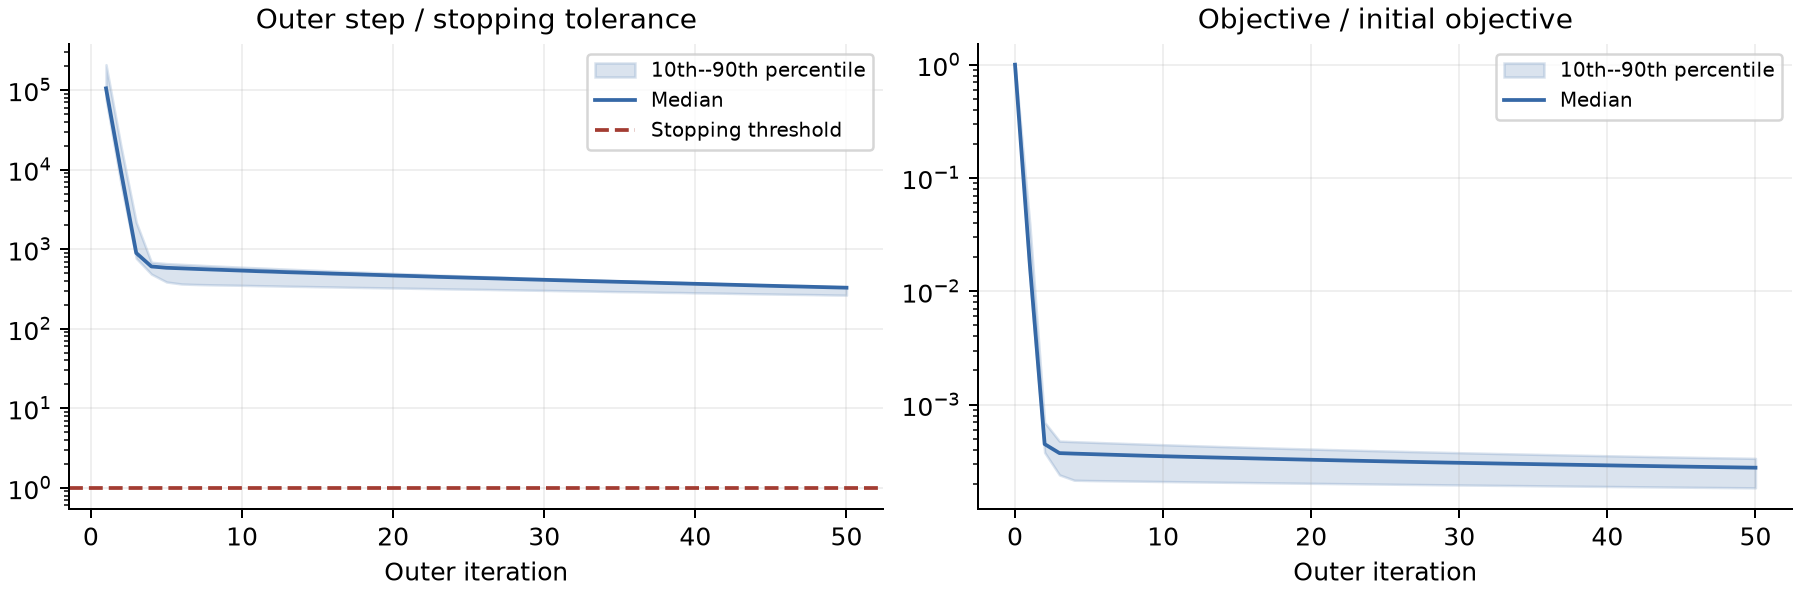
\includegraphics[width=\linewidth]{figures/convergence.png}
\caption{Saved optimization histories. The left panel shows why the outer convergence test was not met. The right panel shows substantial objective reduction, which is a different diagnostic.}\end{figure}
The mean reduction from initial to final native objective was 99.9731\%. Nevertheless, the last outer update still reduced it by a median 0.4449\% (range 0.1921--0.5340\%). No objective-gap lower bound was computed. Small link residuals or a large decrease from a poor start do not establish convergence.

At the final iterates, the mean native data term was 372.4 and mean weighted DCT penalty was 239,386.1. This describes the final objective composition, not a causal explanation of the poor maps. Initialization, transferred weights, sparse geometry and iteration budget have not been isolated experimentally.
\clearpage
\section{Accuracy against the existing methods}
The benchmark contains 100 patches, with 160,000--495,616 pixels (mean 269,491) and 938--1,995 valid links. All seven methods use the same patch set. Results below reproduce the tables already generated for the Roy-inclusive manuscript from its analysis cache. The earlier builder checked all 700 field-level metric records against the saved reconstruction arrays.

For ground truth $g$ and estimate $u$, define
\[
 \mathrm{RMSE}=\sqrt{N^{-1}\sum_i(u_i-g_i)^2},\qquad
 B=N^{-1}\sum_i(u_i-g_i),
\]
\[
 r=\frac{\sum_i(u_i-\bar u)(g_i-\bar g)}
 {\sqrt{\sum_i(u_i-\bar u)^2\sum_i(g_i-\bar g)^2}}.
\]
Compute these within each patch, then report the mean and sample standard deviation across patches. Every patch has equal weight; this is not one pooled-pixel RMSE.
\begin{table}[H]
\centering\small
\begin{tabular}{lrrr}
\toprule
Method & RMSE & Signed bias & Pearson $r$ \\
\midrule
IDW & $1.307\pm 1.241$ & $0.034\pm 0.298$ & $0.866\pm 0.060$ \\
ILDW & $1.239\pm 1.188$ & $0.047\pm 0.263$ & $0.878\pm 0.055$ \\
Solver(ILDW) & $1.059\pm 1.198$ & $0.040\pm 0.236$ & $0.918\pm 0.056$ \\
Solver(GT) & $0.503\pm 0.371$ & $0.009\pm 0.030$ & $0.961\pm 0.032$ \\
Convex solver & $0.845\pm 0.807$ & $0.023\pm 0.075$ & $0.940\pm 0.035$ \\
Homotopy solver & $0.845\pm 0.807$ & $0.023\pm 0.075$ & $0.940\pm 0.035$ \\
Roy DCT (limited) & $3.554\pm 1.865$ & $-2.443\pm 0.786$ & $0.165\pm 0.060$ \\
\bottomrule
\end{tabular}
\caption{Whole-patch metrics: mean $\pm$ sample standard deviation across 100 patches, with equal patch weights. RMSE and bias are in mm/h. Roy DCT denotes the nonlinear adaptation at its iteration limit; Solver(GT) uses privileged ground-truth initialization.}
\label{tab:patch_map_metrics}
\end{table}
Solver(ILDW) is the existing nonlinear optimizer initialized from ILDW; Solver(GT) uses ground-truth initialization and is a privileged reference, not an operational method. Convex and homotopy are the existing repository variants. Roy DCT denotes the nonlinear, iteration-limited adaptation throughout.
\begin{table}[H]
\centering\small
\begin{tabular}{lrrrr}
\toprule
Method vs. IDW & Wins:losses & $\overline{\Delta}$ & $p$ (one-sided) & 99\% upper bound \\
\midrule
ILDW & 97:3 & -0.068 & 2.4e-12 & -0.047 \\
Solver(ILDW) & 98:2 & -0.248 & 6e-21 & -0.198 \\
Solver(GT) & 100:0 & -0.804 & 2.2e-11 & -0.547 \\
Convex solver & 100:0 & -0.461 & 1.9e-15 & -0.344 \\
Homotopy solver & 100:0 & -0.461 & 1.9e-15 & -0.344 \\
Roy DCT (limited) & 0:100 & 2.247 & 1 & 2.438 \\
\bottomrule
\end{tabular}
\caption{Paired patchwise RMSE comparison, with $\Delta=\mathrm{RMSE}_{s}-\mathrm{RMSE}_{IDW}$. Negative differences favor the method. Tests use the alternative $E[\Delta]<0$; values are unadjusted for multiple comparisons. Iteration-limited Roy outputs are retained.}
\label{tab:paired-rmse-t-test}
\end{table}
The paired tests use 100 patchwise differences. The one-sided $p$ value of one for Roy means no evidence for the stated alternative (lower RMSE than IDW); it does not mean equal performance. The 99\% upper bound is $\bar\Delta+t_{0.99,99}s_\Delta/\sqrt{100}$. Spatial or temporal dependence between patches can weaken nominal test calibration; these are descriptive benchmark comparisons without multiple-testing adjustment.
\clearpage
\section{Wet/dry classification and attenuation agreement}
A pixel is wet when its rainfall is at least 0.6 mm/h, and dry otherwise. FP/all and FN/all divide by all pixels in a patch; FP/dry divides by true dry pixels, FN/wet by true wet pixels. Rates are averaged patchwise, with conditional denominators respected. This threshold is an evaluation convention; its numerical equality to the initial constant rainfall is not an optimization constraint.
\begin{table}[H]
\centering\small
\begin{tabular}{lrrrr}
\toprule
Method & FP/all (\%) & FN/all (\%) & FP/dry (\%) & FN/wet (\%) \\
\midrule
IDW & 3.96 & 0.24 & 59.83 & 0.32 \\
ILDW & 3.70 & 0.29 & 56.24 & 0.38 \\
Solver(ILDW) & 3.24 & 0.31 & 46.30 & 0.41 \\
Solver(GT) & 1.14 & 0.21 & 33.05 & 0.26 \\
Convex solver & 2.28 & 0.38 & 40.02 & 0.50 \\
Homotopy solver & 2.28 & 0.38 & 40.07 & 0.50 \\
Roy DCT (limited) & 4.85 & 34.91 & 48.16 & 39.12 \\
\bottomrule
\end{tabular}
\caption{Mean patchwise wet/dry error rates at 0.6 mm/h. False positive: predicted wet, observed dry; false negative: predicted dry, observed wet. Conditional rates use their respective ground-truth classes.}
\label{tab:wet-dry-confusion-merged}
\end{table}
For link lengths $L_\ell>0$ and errors $e_\ell=F_\ell(u)-y_\ell$, the attenuation metrics are
\[
 \mathrm{MAE}_{\rm km}=\frac1M\sum_\ell\frac{|e_\ell|}{L_\ell},\qquad
 J_{\rm atten}=\frac1M\sum_\ell\frac{e_\ell^2}{L_\ell}.
\]
\begin{table}[H]
\centering\small
\begin{tabular}{lrr}
\toprule
Method & Attenuation MAE (dB/km) & $J_{\mathrm{atten}}$ (dB$^2$/km) \\
\midrule
IDW & 0.0503 & 0.0528 \\
ILDW & 0.0136 & 0.0042 \\
Solver(ILDW) & 0.00207 & 0.000295 \\
Solver(GT) & 0.00129 & 4.95e-05 \\
Convex solver & 0.00107 & 3.35e-05 \\
Homotopy solver & 0.000747 & 1.33e-05 \\
Roy DCT (limited) & 0.000388 & 9.06e-07 \\
\bottomrule
\end{tabular}
\caption{Mean patchwise attenuation errors, evaluated consistently for all methods using the actual ITU forward model. $J_{\mathrm{atten}}=M^{-1}\sum_\ell(\widehat A_\ell-A_\ell)^2/L_\ell$. This comparison metric is not the full native objective of Roy DCT.}
\label{tab:attenuation-fit-summary}
\end{table}
Roy's saved fields have the smallest values of these attenuation metrics but the largest mean rainfall RMSE in this comparison. Sparse path measurements leave many field configurations weakly constrained. Therefore a close match to link attenuation does not imply a close match to rainfall everywhere. The strong negative rainfall bias is visible in Table~\ref{tab:patch_map_metrics} and is not visible in a centered Taylor diagram.

The generic cache objective summary does not recognize the Roy native objective. Its generic weighted total should not be interpreted as Eq.~\eqref{eq:objective}; use \texttt{fun}, \texttt{data\_term}, and \texttt{coefficient\_l1} in Roy's saved diagnostics.
\clearpage
\section{Runtime and what is comparable}
\begin{table}[H]\centering\small\begin{tabular}{llrrrr}\toprule Method & Scope & Mean & Median & Min--max & Total\\\midrule
IDW & End-to-end & 7.53 & 7.10 & 4.01--14.18 & 0.209 h \\
ILDW & End-to-end & 18.69 & 18.25 & 8.67--38.19 & 0.519 h \\
Convex & End-to-end & 76.03 & 71.31 & 32.76--153.12 & 2.112 h \\
Convex & Optimizer & 57.00 & 51.15 & 17.61--118.61 & 1.583 h \\
Roy DCT & Optimizer & 168.77 & 152.32 & 71.95--423.60 & 4.688 h \\
Solver(ILDW) & Not recorded & -- & -- & -- & -- \\
Solver(GT) & Not recorded & -- & -- & -- & -- \\
Homotopy & Not recorded & -- & -- & -- & -- \\
\bottomrule\end{tabular}
\caption{Saved runtime records for the same 100 patch identifiers. Per-patch mean, median and range are in seconds; total is in hours. Missing timings are not estimated.}\end{table}
\textbf{The two Convex rows measure the same runs, not different methods.} End-to-end time (mean 76.03 s) contains input loading, setup, initialization, optimization, diagnostics and saving. Optimizer time (mean 57.00 s) is the nested numerical optimization call alone. Do not add them: their mean difference, 19.03 s, is the surrounding work.

\textbf{Two limits on comparison with Roy.} First, Roy's optimizer-only time should be compared with the Convex optimizer row, not its end-to-end row. Second, the stopping conditions differ: the convex benchmark reports convergence, whereas Roy exhausted its outer iteration budget. This is not a comparison of time to the same convergence or accuracy target.

Roy's total optimizer time was 16,876.805 seconds, or \textbf{4 h 41 min 17 s}. The median was 152.324 s and interquartile range 120.120--200.912 s. Timing starts immediately before the outer loop and includes its inner solves, Jacobians, line search, and final prediction/diagnostic calculation up to the timer read. It excludes input loading, operator setup, the initial objective evaluation, and output writing. Roy end-to-end batch wall time was not recorded.

The prior IDW, ILDW and convex timing benchmarks record end-to-end wall times including loading, initialization, reconstruction, diagnostics and writing. Convex optimizer time covers its \texttt{scipy.optimize.minimize} call. These are separately executed timing runs, not timestamps extracted from the accuracy-cache reconstruction run. Their patch identities match all 100 Roy patches.

The prior benchmark metadata identify an Apple M2 MacBook Air (8-core CPU, 8 GB memory), Python 3.14.3, NumPy 2.5.0 and SciPy 1.18.0, with one solver worker and one patch worker. Roy's configuration also specifies one worker of each kind, but its saved diagnostics do not record hardware or package versions. Do not treat the runtime table as a controlled same-session hardware benchmark. Furthermore, stopping rules differ and Roy did not converge: these are costs of the saved procedures, not time to a shared accuracy or optimality target.

No runtime record was found for Solver(ILDW), Solver(GT), or homotopy in the available solution metadata or timing files. Iteration counts cannot reliably substitute for their runtimes.
\clearpage
\section{Memory and reproducibility implications}
For $N=250{,}000$, a dense $N\times N$ float64 basis would require $500$ GB (about $466$ GiB), before work arrays. We instead apply DCT and inverse DCT in $O(N\log N)$ time and use sparse link operators. Storage scales roughly with pixels, links and nonzero link--pixel intersections, rather than $N^2$. Each CG matrix action costs $O(\operatorname{nnz}(J_k)+N)$.

The project declares NumPy and SciPy dependencies; its lock file specifies versions. That lock is a reproducibility target, not evidence of the versions used for a past run. Save a package freeze, hardware metadata, full runtime scope and input hashes for future comparisons. The solver uses deterministic constant initialization and has no random coefficient initialization.
\clearpage
\section{Taylor diagrams: definitions and combined normalized view}
Radius shows spatial standard deviation; angle is $\arccos(r)$, where $r$ is correlation with ground truth. Distance to the reference point is centered RMSE. Means are removed, so bias is excluded.

The combined normalized point gives every patch equal weight after division by its ground-truth standard deviation. If $g_i,f_i,c_i$ are within-patch truth SD, estimate SD and covariance, then
\[
 G=1,\qquad F=\sqrt{\langle f_i^2/g_i^2\rangle},\qquad
 C=\langle c_i/g_i^2\rangle,\qquad r=C/F.
\]
Here $F$ is radius and brackets mean an average over the 100 patches.
\begin{figure}[H]\centering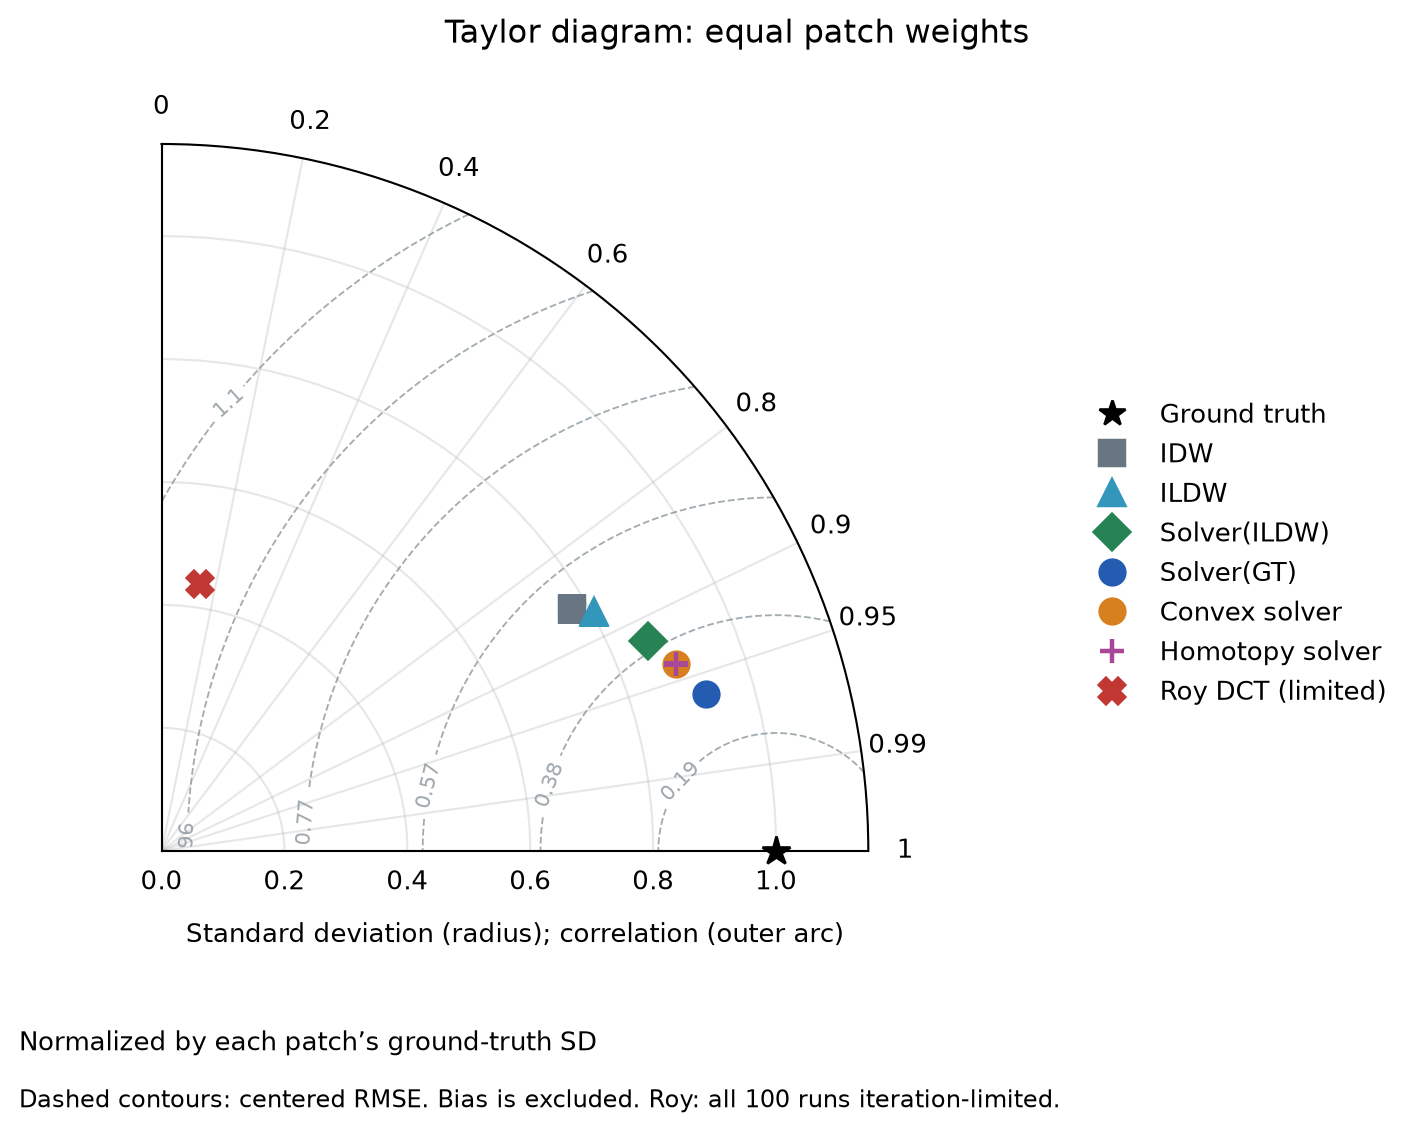
\includegraphics[width=\linewidth]{figures/combined_normalized.png}
\caption{One normalized point per solver, based on 100 patches. The star is ground truth. Radius measures relative spatial variability; angle measures correlation; dashed contours measure centered error. Mean bias is excluded.}\end{figure}
\clearpage
\section{Combined Taylor diagram in physical units}
The physical-units diagram combines within-patch moments with equal patch weights:
\[
 G=\sqrt{\langle g_i^2\rangle},\qquad F=\sqrt{\langle f_i^2\rangle},\qquad
 C=\langle c_i\rangle,\qquad r=C/(GF).
\]
Radius is $F$ in mm/h; centered RMSE is $\sqrt{F^2+G^2-2C}$. This aggregate correlation differs from the mean patch correlation in the accuracy table.
\begin{figure}[H]\centering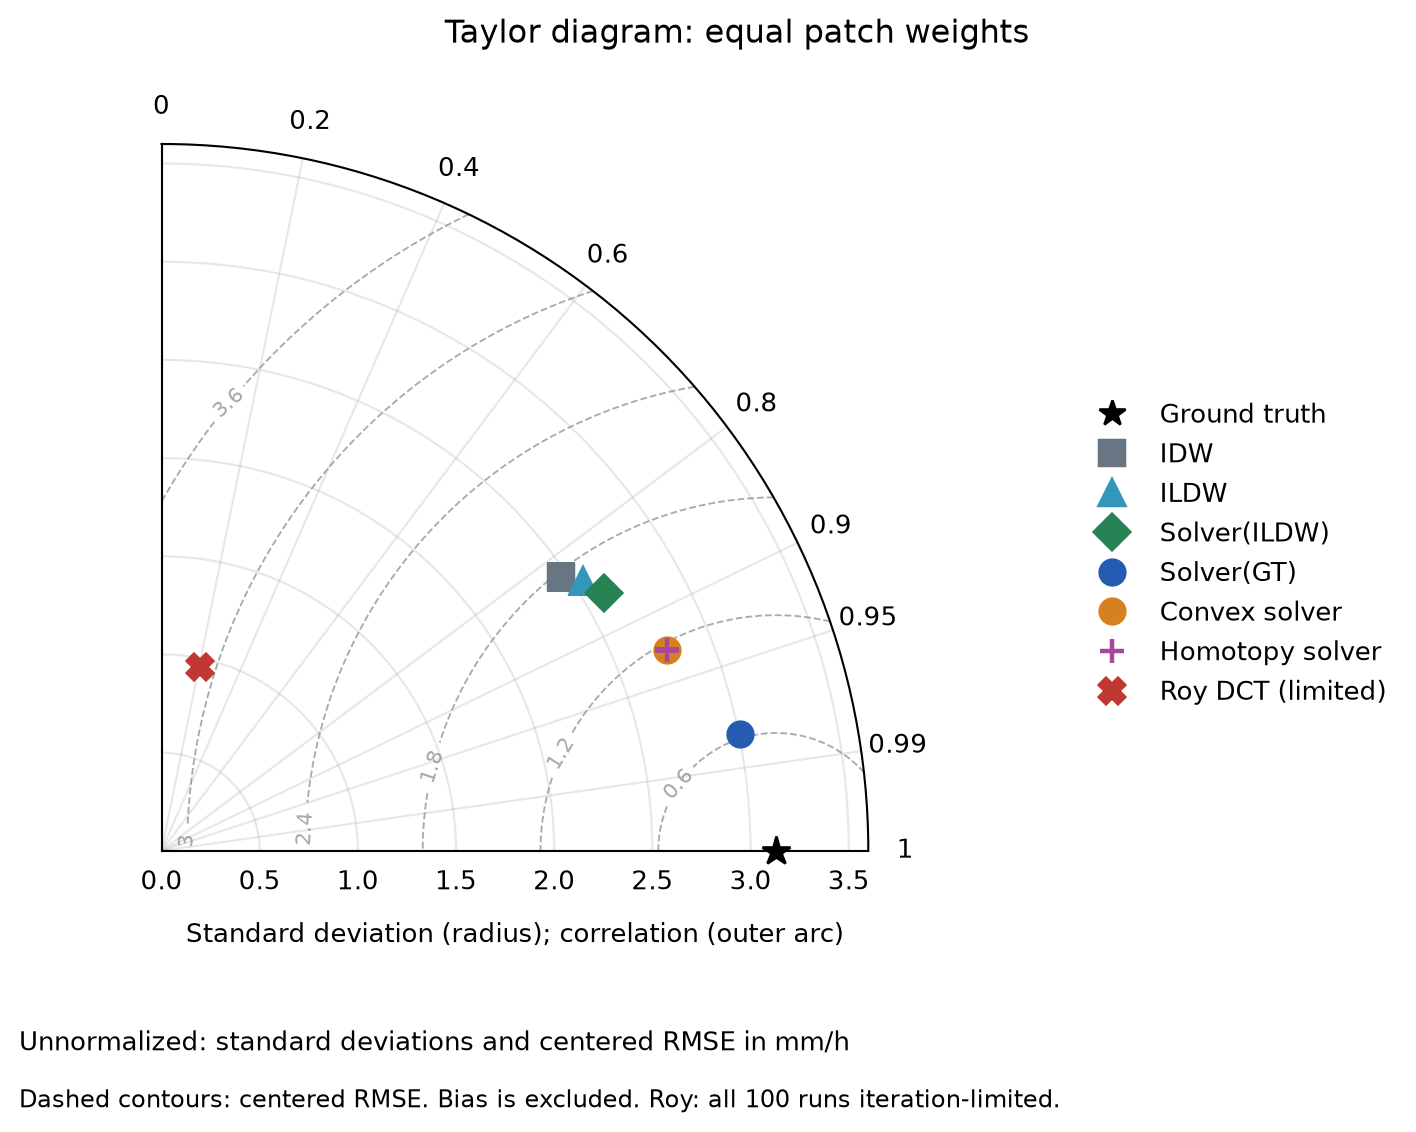
\includegraphics[width=\linewidth]{figures/combined_unnormalized.png}
\caption{One point per solver in mm/h. Convex and homotopy nearly coincide. A small radius alone is not desirable: the estimate should also reproduce the ground-truth variability and correlation.}\end{figure}
Roy's limited-run results have low spatial variability and low correlation; the map bias must additionally be read from the accuracy table. These diagrams summarize saved output quality and do not diagnose why the optimizer produced those fields.
\clearpage
\section{Individual-patch Taylor diagrams}
Each panel shows 100 individual patches. A patch has radius $f_i/g_i$, angle $\arccos(r_i)$ and reference radius one. All panels use the same scale; mean bias is excluded.
\begin{figure}[H]\centering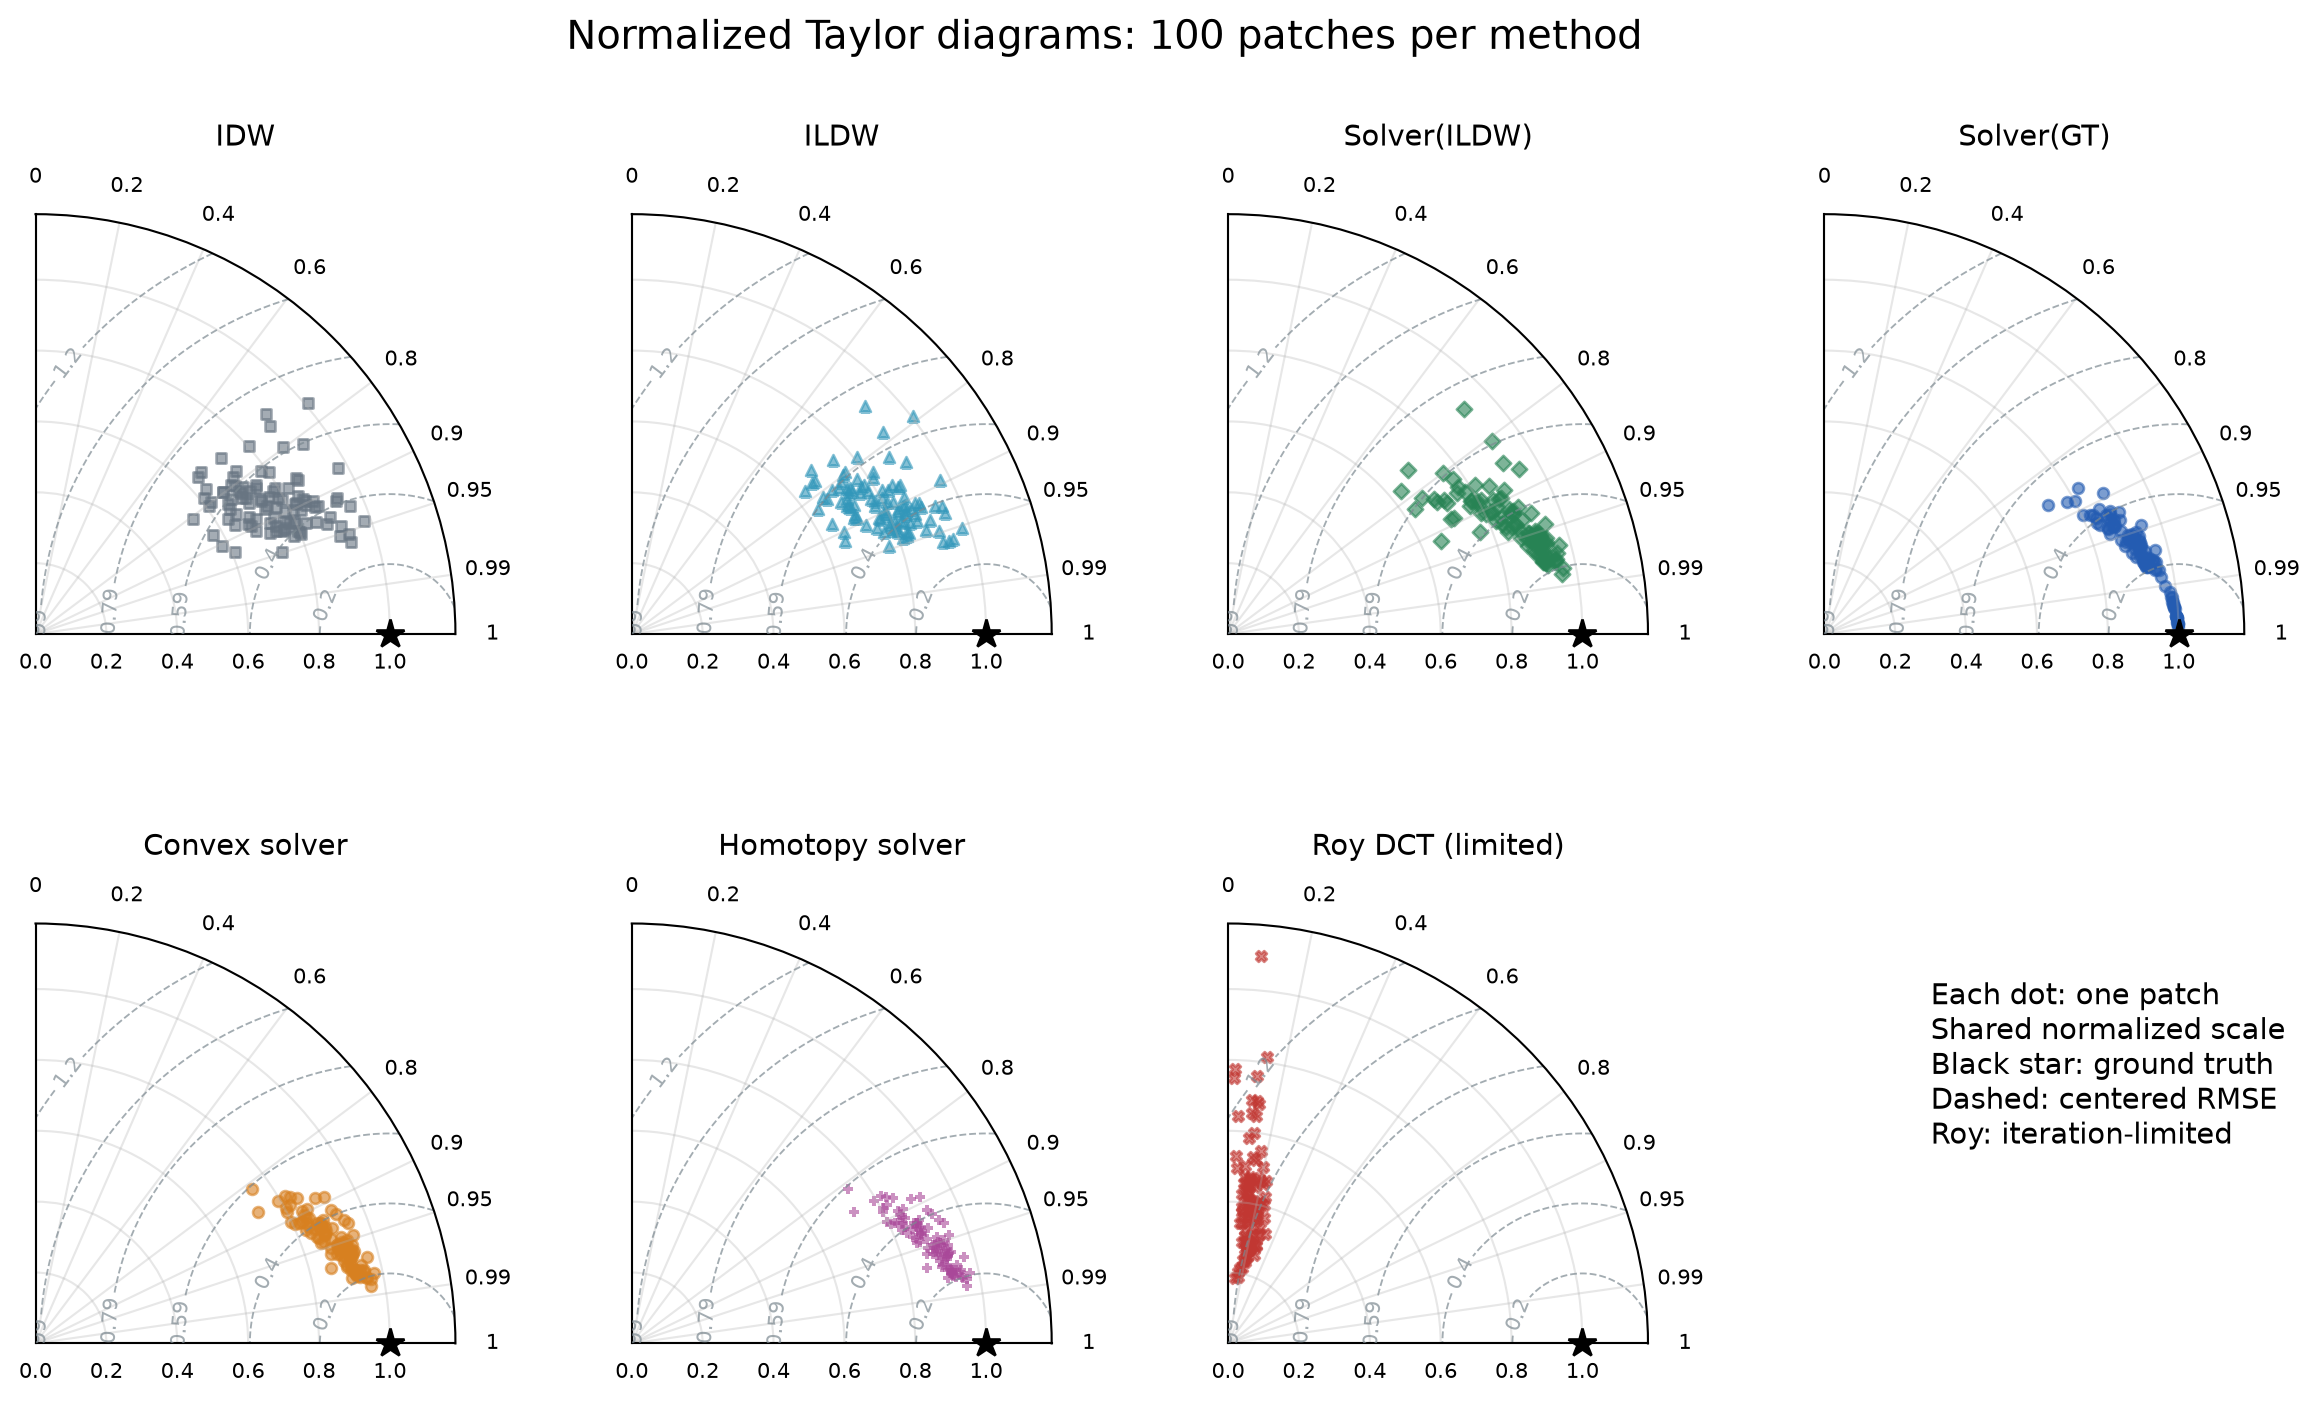
\includegraphics[width=\linewidth]{figures/patch_clouds_normalized.png}
\caption{Normalized individual-patch Taylor points. Each panel uses the same axes, so the distributions can be compared directly. All Roy points come from runs stopped at the outer iteration cap.}\end{figure}
\clearpage
\section{Audit trail, limitations and next experiments}
\textbf{Evidence sources.} The method was checked against the current implementation and the saved run metadata. The quantitative audit reads 100 Roy \texttt{\_optinfo.json} files, the existing runtime summaries/CSVs, and the tables and Taylor figures generated for the Roy-inclusive manuscript. It does not modify the solver, original manuscript, cache, or existing results.

\begin{tabular}{p{.24\linewidth}p{.69\linewidth}}\toprule
Item & Repository-relative location\\\midrule
Solver & \path{Compute-Link-Attenuations/cml_attenuation/solvers/solve_rain_roy_dct.py}\\
Run configuration & \path{Compute-Link-Attenuations/HundredPatches/pipeline/batch_solve_roy_dct.yaml}\\
Saved Roy runs & \path{Compute-Link-Attenuations/HundredPatches/pipeline/solutions/sol_dir_roy_dct_nonlinear/}\\
Analysis cache & \path{Compute-Link-Attenuations/HundredPatches/pipeline/batch_analyze_output_roy_dct/stats_report_cache.json}\\
Other timings & \path{Compute-Link-Attenuations/HundredPatches/pipeline/timing/all_methods/}\\
Comparison manuscript & \path{output/journal_roy_dct/Journal_with_Roy_DCT.tex}\\\bottomrule
\end{tabular}

The source bundle includes this \LaTeX{} file, extracted tables, figures, \texttt{run\_summary.json}, per-patch convergence/runtime CSV, Taylor statistics, and the audit script. The summary records SHA-256 hashes of the solver, configuration and comparison manuscript at audit time. Run \texttt{latexmk -pdf roy\_dct\_solver\_note.tex} in the bundle directory to compile. The audit script additionally requires the repository and its saved data at their existing paths.

\textbf{Interpretation limits.} There is no nonlinear global-optimality certificate, no saved objective-gap bound, and no CG residual history. The outer step ratios quantify failure of a particular stopping test, not distance from truth or from an optimum. At dry pixels, safeguarded derivatives qualify exact stationarity interpretations. The current objective weights were transferred without calibration; the constant DCT coefficient is penalized, so the prior can affect total rainfall as well as spatial detail. Link data are highly underdetermined relative to pixel counts. The operational-data effects excluded by this simulated benchmark should not be inferred from its accuracy tables.

\textbf{Useful next experiments.} First increase the outer budget on representative patches while saving all diagnostics, and test tighter inner tolerances to assess the effect of inexact subproblem solves. Then compare constant, IDW and ILDW initialization under matched stopping criteria. Finally, tune the effective regularization $\beta$ on held-out patches and repeat runtime measurements with matched hardware and timing scope. None of these experiments has been performed for this note.
\begin{thebibliography}{9}
\bibitem{roy} V. Roy, S. Gishkori and G. Leus. Dynamic rainfall monitoring using microwave links. \emph{EURASIP Journal on Advances in Signal Processing}, 2016:77. \url{https://doi.org/10.1186/s13634-016-0367-6}. Especially Eqs.~(26)--(27) and Section 5.3.3.
\bibitem{osqp} OSQP documentation. Python interface. \url{https://osqp.org/docs/interfaces/python.html}.
\bibitem{cg} SciPy documentation. \texttt{scipy.sparse.linalg.cg}. \url{https://docs.scipy.org/doc/scipy/reference/generated/scipy.sparse.linalg.cg.html}.
\bibitem{dct} SciPy documentation. \texttt{scipy.fft.dctn}. \url{https://docs.scipy.org/doc/scipy/reference/generated/scipy.fft.dctn.html}.
\end{thebibliography}
\end{document}
